% pyFormex manual
%
\documentclass[a4paper]{manual}
\let\pyurl\url
\let\url\relax
\usepackage{hyperref}
%\usepackage[latex2html]{hyperref}
%\usepackage[latex2html,pdftex]{hyperref}
\usepackage{html}
\usepackage{xspace}
\usepackage{graphicx}
%\usepackage[pdftex]{graphicx}
\title{pyFormex manual}
\author{Tim Neels, Benedict Verhegghe}
\release{0.3-alpha}
\setshortversion{0.3}
\newcommand{\pyformex}{pyFormex\xspace}
\newcommand{\website}{http://pyformex.berlios.de}
\newcommand{\websitelink}{\pyurl{\website}}

\begin{document}
\maketitle
\chapter{Introduction}
\label{cha:introduction}

\section{What is \pyformex{}?}
\label{sec:what-pyformex}
You probably expect to find here a short definition of what \pyformex is and what it can do for you. I may have to disappoint you: describing the essence of \pyformex in a few lines is not an easy task to do, because the program can be (and is being) used for very different tasks. So I will give you two answers here: a short one and a long one.

The short answer is that \pyformex{} is a program to \emph{generate large structured sets of coordinates by means of subsequent mathematical transformations gathered in a script.}
If you find this definition too dull, incomprehensible or just not descriptive enough, read on through this section and look at some of the examples in this manual and on the \pyformex{} website\footnote{\websitelink}. You will then probably have a better idea of what \pyformex{} is. 

The initial intention of \pyformex{} (and probably still its main use) was the rapid design of three-dimensional wireframe structures with a configuration that can easier be obtained through mathematical description than through interactive generation of its subparts and assemblage thereof.

The example of the stent\footnote{A stent is a tube-shaped structure that is e.g. used to reopen (and keep open) obstructed blood vessels.} in the figure below illustrates this clearly. 

\begin{figure}[h]
  \begin{makeimage}
  \end{makeimage}
  \centering
  %\htmlimage{scale=0.5}
  \begin{latexonly}
  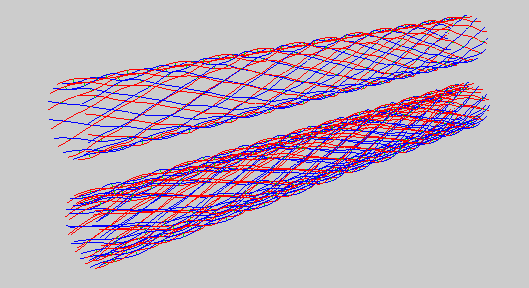
\includegraphics[width=12cm]{../../examples/WireStent}
  \end{latexonly}
  \begin{htmlonly}
    %\hyperimage{../../examples/WireStent.png}
    \htmladdimg{../../../examples/WireStent.png}
  \end{htmlonly}  \caption{WireStent example.}
\end{figure}


The structure has 


\section{History}
\label{sec:history}

\section{Quick tutorial for the \pyformex{} GUI}
\label{sec:gui-tutorial}
In the current version () the GUI mainly serves the following purposes:
\begin{itemize}
\item Display a structure in 3D. This includes changing the viewpoint, orientyation and viewing distance. Thus you can interactively rotate, translate, zoom.
\item Save a view in one of the supported image formats. Most of the images in this manual and on the \pyformex{} website were created that way. 
\item Changing \pyformex settings (though there aren't many yet that can be changed through the GUI).
\item Running \pyformex scripts, possibly starting other programs and display their results.
\end{itemize}

The GUI does not (yet) provide a means to interactively design a structure, select parts of a structure or set/show information about (parts of) the structure. Designing a structure is done by writing a small script with the mathematical expressions needed to generate it. Any text editor will be suitable for this purpose. The author uses XEmacs, but this is just a personal preference. 
A Python aware editor is preferable though, because that is the language used in pyFormex scripts.
A \pyformex editor integrated into the GUI remains on our TODO list, but it certainly has not our top priority, because general purpose editors are adequate for most of our purposes. 

The best way to learn to use pyFormex is by studying and changing some of the examples. I suggest that you first take a look at the examples included in the pyFormex GUI and select those that display structures that look interesting to you. Then you can study the source code of those examples and see how the structures got built. 
When starting up, \pyformex reads through the Examples directory (this is normally the 'examples' subdirecty located under the pyformex installation dir).  
\menuselection{Examples \sub WireStent}


\section{Quick scipy tutorial}
\label{sec:scipy-tutorial}

%%%%%%%%%%%%%%%%%%%%%%%%%%%%%%%%%%%%%%%%%%%%%%%%%%%%%%%%%%%%%%%%%%%%%%%%%%%
\chapter{formex --- the base module}
{\label{cha:formex}

This module contains all the basic functionality for creating, structuring and transforming sets of coordinates.

\begin{classdesc}  {Formex}{data=[[[]]],prop=None}
A class to hold a structured set of coordinates. A \class{Formex} is a threedimensional array of float values. The array has a shape \code{(nelems,nnodel,3)}. Each slice \code{[i,j]} of the array contains the three coordinates of a point in space. We will also call this a \emph{node}. Each slice \code{[i]} of the array contains a connected set of nnodel points: we will refer to it as an \emph{element}. 

It is up to the user on how to interprete this connection: two connected nodes will usually represent a line segment between these two points. An element with three nodes however could just as well be interpreted as a triangle or as a (possibly curved) line. And if it is a triangle, it could be either the circumference of the triangle or the part of the plane inside that circumference. As far as the Formex class concerns, each element is just a set of points. 

All elements in a \class{Formex} must have the same number of points, but you can construct \class{Formex} instances with any (positive) number of nodes per element. When \code{nnodel==1}, the \class{Formex} contains only unconnected nodes (each element is just one point).

One way of attaching other data to the \class{Formex}, is by the use of the 'property' attribute. The property is an array holding one integer value for each of the elements of the Formex. The use of this property value is completely defined by the user. It could be a code for the type of element, or for the color to draw this element with. Most often it will be used as an index into some other (possibly complex) data structure holding all the characteristics of that element. 

By including this property index into the Formex class, we make sure that when new elements are constructed from existing ones, the element properties are automatically propagated.

\end{classdesc}

\begin{memberdesc}  [array]{f}
A threedimensional array of float values. The array has a shape (nelems,nnodel,3). Each slice [i,j] of the array contains the three coordinates of a point in space. We will also call this a \emph{node}. Each slice [i] of the array contains a connected set of nnodel points: we will refer to it as an \emph{element}. It is up to the user on how to interprete this connection: two connected nodes will usually represent a line segment between these two points. An element with three nodes however could just as well be interpreted as a triangle or as a (possibly curved) line. And if it is a triangle, it could be either the circumference of the triangle or the part of the plane inside that circumference.   
\end{memberdesc}



\end{document}
